\documentclass[border=10pt]{standalone}

\usepackage{tikz}
\usepackage{tikzsymbols}
\usetikzlibrary{calc,patterns,shapes.geometric}

\def\centerarc[#1](#2)(#3:#4:#5){\draw[#1] ($(#2)+({#5*cos(#3)},{#5*sin(#3)})$) arc (#3:#4:#5);}

\begin{document}
	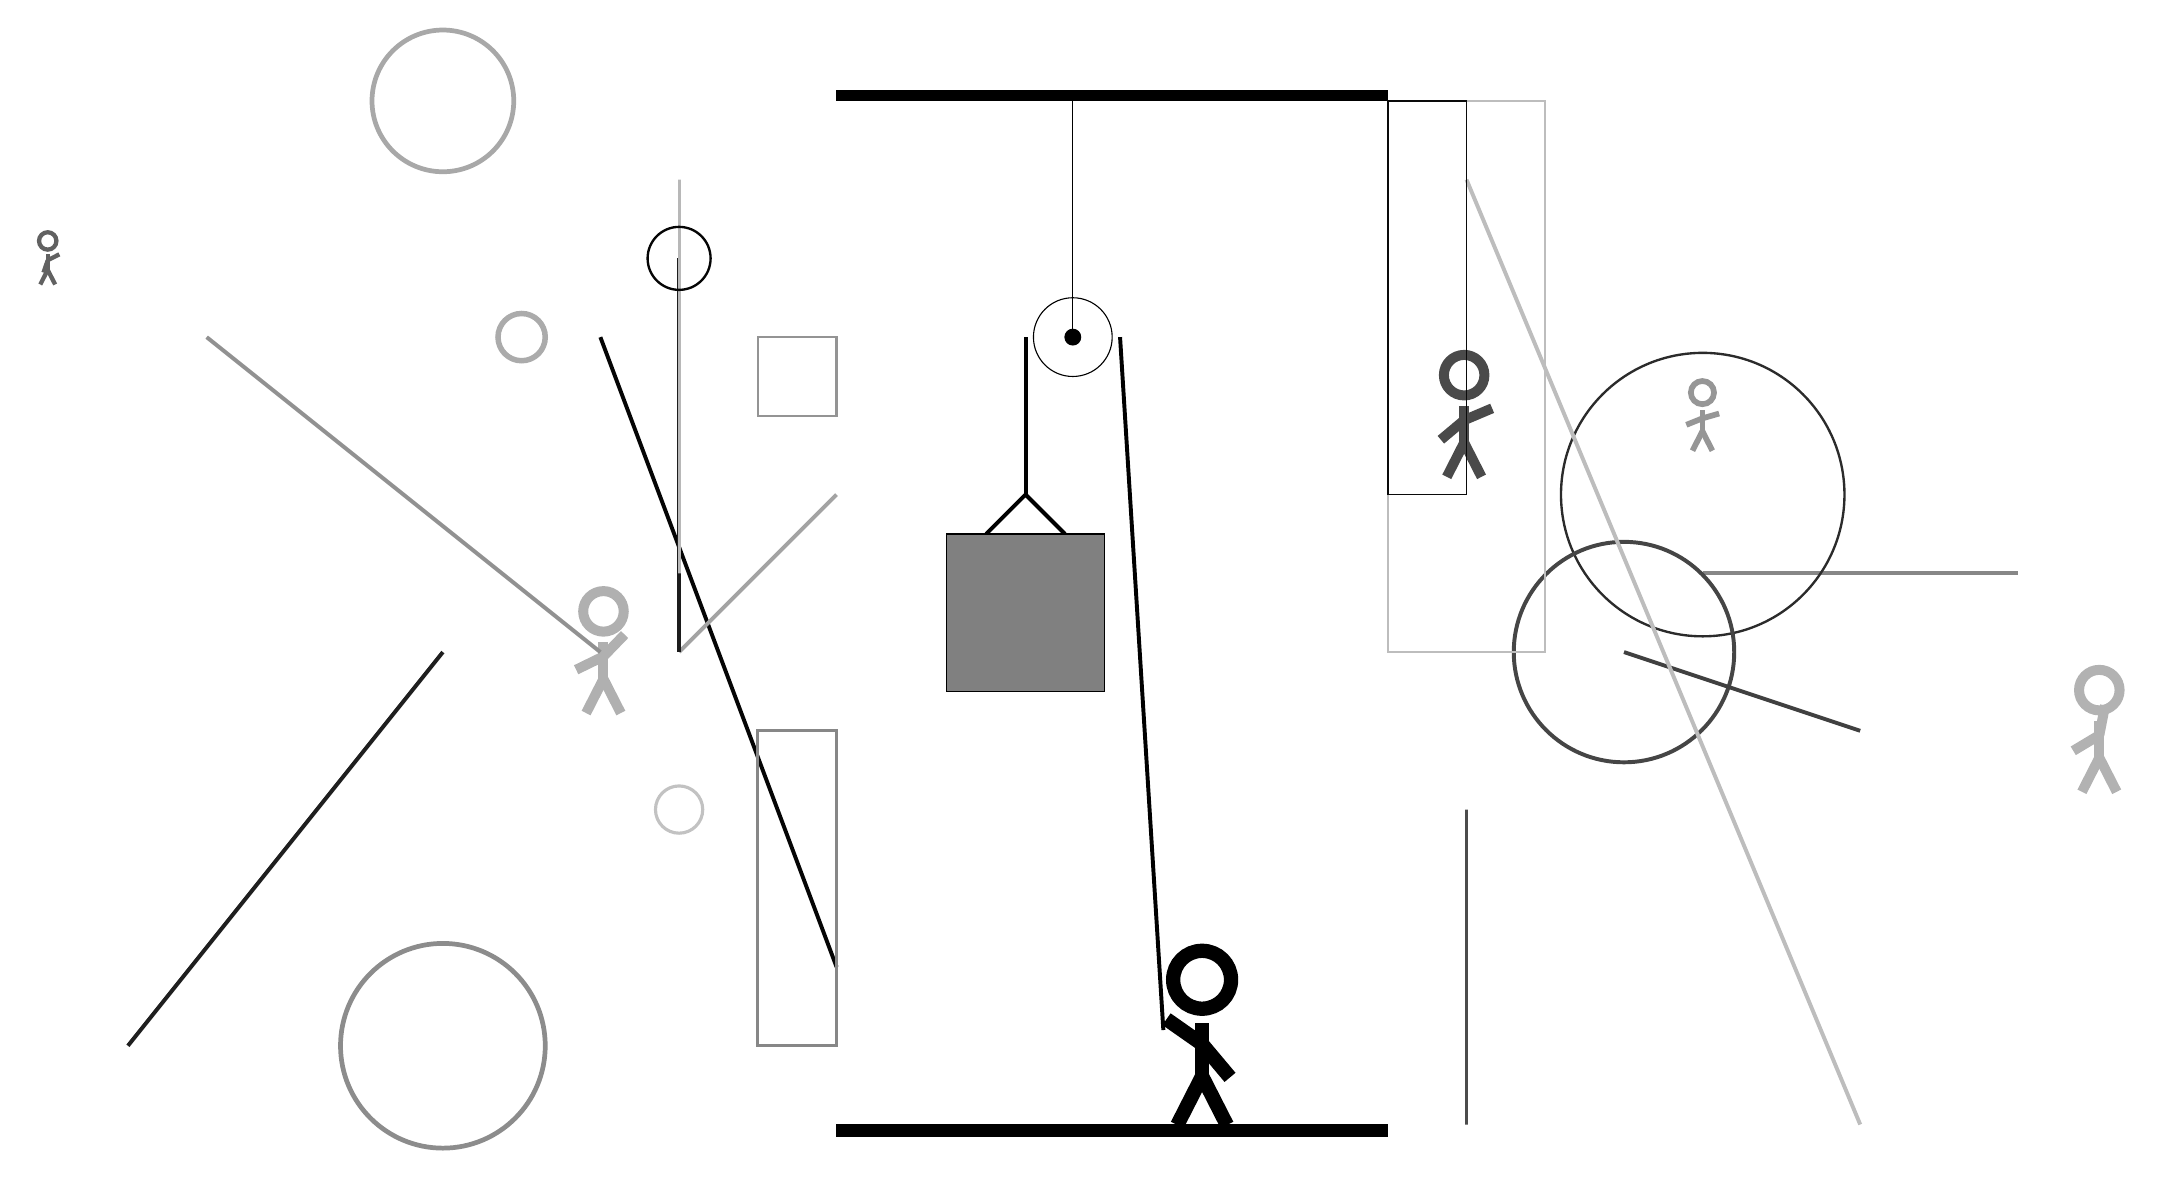
\begin{tikzpicture}
		%%%%% START %%%%%
		
		\draw[fill=black] (-2, 10) rectangle (5, 10.125);
		
		\draw (1, 7) circle (0.5);
		\draw[fill=black] (1, 7) circle (0.1);
		\draw (1, 10) -- (1, 7);
		
		\draw[line width=0.5mm] (-0.1, 4.5) -- (0.4, 5.0) -- (0.9, 4.5);
		\draw[fill=black!50] (-0.6, 4.5) rectangle (1.4, 2.5);
		
		\draw[line width=0.5mm] (0.4, 7) -- (0.4, 5.0);
		\centerarc[line width=0.5mm](1, 7)(0:180:0.6);
		\draw[line width=0.5mm](1.6, 7) -- (2.15, -1.8);
		
		\draw[line width=0.5mm, color=black!98](-2, -1) -- (-5, 7);
		
		\draw [line width=0.6mm, color=black!45](-7, -2) circle (1.3);
		\node[line width=0.5mm, color=black!30] at (14, 2) {\Strichmaxerl[7][31][79]};
		\draw[line width=0.5mm, color=black!47](9, 4) -- (13, 4);
		
		\draw [line width=0.3mm, color=black!83](9, 5) circle (1.8);
		
		\draw[line width=0.5mm, color=black!36](-2, 5) -- (-4, 3);
		\draw [line width=0.4mm, color=black!24](-4, 1) circle (0.3);
		\draw [line width=0.5mm, color=black!73](8, 3) circle (1.4);
		\draw[line width=0.3mm, color=black!26] (7, 3) rectangle (5, 10);
		
		\draw[line width=0.5mm, color=black!75](8, 3) -- (11, 2);
		\draw[line width=0.5mm, color=black!88](-7, 3) -- (-11, -2);
		\node[line width=0.2mm, color=black!71] at (6, 6) {\Strichmaxerl[7][40][23]};
		\node[line width=0.6mm, color=black!41] at (9, 6) {\Strichmaxerl[4][22][16]};
		
		\draw [line width=0.6mm, color=black!34](-7, 10) circle (0.9);
		\draw[line width=0.5mm, color=black!70] (6, 1) rectangle (6, -3);
		\node[line width=0.6mm, color=black!31] at (-5, 3) {\Strichmaxerl[7][26][46]};
		\draw[line width=0.3mm, color=black!42] (-2, 7) rectangle (-3, 6);
		\draw[line width=0.5mm, color=black!89](-4, 8) -- (-4, 3);
		\draw [line width=0.7mm, color=black!36](8, 1) circle (0.0);
		\draw[line width=0.5mm, color=black!26](6, 9) -- (11, -3);
		\draw[line width=0.4mm, color=black!47] (-3, 2) rectangle (-2, -2);
		
		\draw [line width=0.7mm, color=black!33](-6, 7) circle (0.3);
		\draw[line width=0.2mm, color=black!96] (5, 10) rectangle (6, 5);
		\draw[line width=0.4mm, color=black!28] (-4, 9) rectangle (-4, 4);
		\node[line width=0.3mm, color=black!62] at (-12, 8) {\Strichmaxerl[3][71][27]};
		
		\draw [line width=0.3mm, color=black!98](-4, 8) circle (0.4);
		\draw[line width=0.5mm, color=black!43](-5, 3) -- (-10, 7);
		
		\node at (2.6, -1.9) {\Strichmaxerl[10][-35][-50]};
		
		\draw[fill=black] (-2, -3) rectangle (5, -3.15);
		
		%%%%% END %%%%%
	\end{tikzpicture}
\end{document}